% Copyright (c) 2008-2009 solvethis
% Copyright (c) 2010-2011 Casper Ti. Vector
% Public domain.

\chapter{验证平台使用样例设计}
	本章会通过两个实际的物理层WiFi安全研究的样例,进一步说明GRTSEC平台的使用场景和方法,
	同时,用户也可以基于这些使用样例开展自己的研究。
	在\ref{sec:demo_fake_wifi}节会介绍如何使用GRTSEC搭建伪装WiFi,并用伪装WiFi发起钓鱼攻击,获取用户的敏感信息,
	在\ref{sec:demo_phy_auth}节会提出一种利用利用硬件指纹技术对不同WiFi设备进行识别的方法。

	\section{搭建伪装AP}\label{sec:demo_fake_wifi}
	身份伪装是很多WiFi攻击的前提和基础,比如DoS攻击、会话劫持、中间人攻击、数据篡改、窃听等\cite{ieeewc10}。
	针对身份伪装的安全研究需要先搭建伪装AP,本节设计了搭建伪装AP的样例,并用伪装AP发起钓鱼攻击,获取用户的敏感信息,

		\subsection{样例背景}
		在北京大学,计算中心为全校师生员工提供了无线校园WiFi,名字是WirelessPKU,遍布教学楼、实验室、食堂等场所。
		WirelessPKU是无密码的开放WiFi,用户连接到WirelessPKU后,首先跳转到一个认证网页,输入网关的账号、密码进行登录,
		登录后才可以继续上网。对于学生来说,网关账号、密码同时也是其他校园网页登录的账号、密码,
		包括信息登记、成绩查询、选课申请等都使用同一套认证系统。
		假如密码泄露会造成巨大的损失,轻则已选的课程被退掉或者成绩泄露,重则学籍信息被篡改,无法毕业。
		在本节,我们将利用GRTSEC搭建AP,伪装成WirelessPKU,并制作一个钓鱼认证网页,用来盗取统一认证账号。

		\subsection{场景设计}
		真实WirelessPKU的AP与伪装AP的分布场景如图\ref{fig:demo_fake_wifi_scenary}所示,
		这张图真实地模拟了北京大学理科五号楼五楼的AP分布,其中AP1、AP2、AP3是北京大学计算中心布置的WirelessPKU的AP,
		GRTSEC摆放在房间1中。假设AP1、AP2、AP3的MAC地址是$MA_1$、$MA_2$、$MA_3$。
		房间1内有个用户,我们称他为小明,在GRTSEC发起伪装之前,小明可以看到信号较强的AP1和信号弱一些的AP2,看不到远处的AP3。
		为了让小明能够连接上GRTSEC,我们将GRTSEC的SSID设置为WirelessPKU,将MAC地址设置为$MA_3$,
		即使小明用MAC地址的白名单来分辨伪装AP也是无法识别的。小明连接上GRTSEC搭建的AP后,会先看到钓鱼认证网页,
		习惯了上网认证的小明会毫无戒心的输入自己的统一认证账号和密码。

		此样例旨在说明设计目标中的两点:可与商用802.11设备实时通信,在这里是与小明的手机相连;
		% 支持自定义数据处理流程,在这里是监听特定包并发送干扰信号;
		可与上层网络协议栈连接,在这里是与应用层的钓鱼认证网页相连。

			\begin{figure}
				\centering
				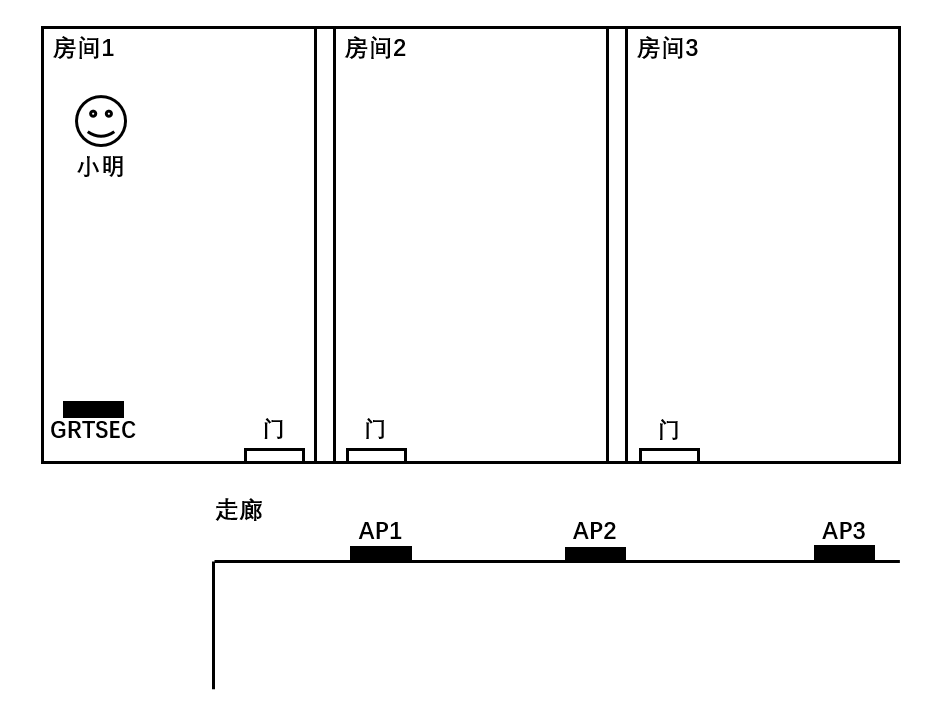
\includegraphics[width=0.7\textwidth]{img/demo_fake_wifi_scenary.png}
				\caption{伪装AP与真实AP分布场景图}
				\label{fig:demo_fake_wifi_scenary}
			\end{figure}

		\subsection{样例实现}
		首先,在上位主机上搭建钓鱼认证网页,钓鱼网页参考了本组张高瀚同学做的网页\cite{zgh17wifi},
		然后,修改主机的网络配置,使网络请求都转跳到钓鱼认证网页,
		最后,将GRTSEC运行在AP模式,等待进入房间1的用户连接。

	\section{利用物理层信息识别不同WiFi设备}\label{sec:demo_phy_auth}
	在802.11协议中,WiFi身份的标识是MAC地址,然而MAC地址非常容易伪装,利用笔记本电脑,
	或者一部root过的安卓手机,搭配一些软件工具,就可以任意修改自己的MAC地址\cite{NetworkSecurity11hacking}。
	在本节,我们提出一种利用物理层信息识别WiFi设备的方法,具体来说,使用物理层信息中的频偏和时钟偏移,识别不同的WiFi设备硬件,
	弥补仅靠MAC地址进行识别的缺陷。

		\subsection{样例背景}\label{subsec:demo_trusted_sta}
		一些用户家里的WiFi偶然被邻居知道了密码,又不想修改密码使自己的全部设备重新输入一次,我们假设这样的一个用户叫小明。
		为了防止邻居的“蹭网”,小明会对路由器进行设置,只允许特定MAC地址的设备连接,目前很多路由器支持这种模式。
		但是,不怀好意的邻居可以监听到小明设备的MAC地址,将自己的设备伪装成小明的设备骗过路由器,继续进行蹭网。
		小明希望做的是对自己的设备进行信任而不是对MAC地址进行信任,在本节,我们利用GRTSEC从接收到的包中提取频偏和时钟偏移,
		生成与WiFi设备对应的硬件指纹,这样小明可以在路由器端选择对特定硬件指纹进行信任,防止邻居继续蹭网。

		本样例主要关注对不同WiFi设备的识别和区分,并不针对无线路由器识别用户设备,实际上这种方法是通用的,
		可用于AP识别STA,可用于识别\ref{sec:demo_fake_wifi}节提出的伪装AP,也可用于STA之间的互相识别。

		\subsection{场景设计}
		我们对AP模式和STA模式的设备进行测试,设计了以下场景。
			\begin{itemize}
				\item 区别不同的STA,使手机和笔记本电脑工作在STA模式,用GRTSEC对这些设备进行区分,
				应用场景是\ref{subsec:demo_trusted_sta}小节提到的防邻居“蹭网”;
				\item 区别不同的AP,在同一地点存在多个同SSID的AP,用GRTSEC进行区分,
				应用场景是识别\ref{sec:demo_fake_wifi}节提出的伪装AP。
			\end{itemize}

		\subsection{样例实现}
		首先,我们利用GRTSEC监听周边WiFi设备发出的包,记录物理层信息,切换多个频道进行记录,
		区别不同的STA时,由于STA不会定时发送beacon包,我们无法获得时钟偏移,只能得到频偏,因此区别不同STA的场景采集的物理层信息是频偏,
		而其他两种场景采集的物理层信息是频偏和时钟偏移。
		然后,我们将记录到的前半部分数据作为训练集,利用KNN(K-nearest neighbors)算法进行建模。
		最后,我们将记录到的后半部分数据作为测试集,用训练好的模型进行区分。
		训练和测试代码都由Python实现。
